\chapter{Vehicle and Track modeling framework}
The goal of the thesis is to select a sufficiently accurate yet computationally tractable model of the vehicle.
There is no single vehicle model that fits all requirements of race engineers. For each problem, a different complexity of the vehicle model is sufficient, e.g.\ for analysis of a power-limit algorithm, the lateral dynamics of the vehicle can be heavily simplified, and simple transcription and solving methods yield sufficient accuracy within a fraction of a second. This is described in Section~\ref{QSS}. Whereas analysis of the torque allocation problem requires the full twin-track model and more computationally expensive transcription and solving methods. Therefore, a vehicle modeling framework is needed to satisfy the needs of different types of analyses.

\section{Graph-centered approach for vehicle modeling}
The structure of the vehicle model has to allow extending or changing components, so that different vehicle concepts can be simulated with minimal coding. The book~\cite{brown_engineering_2006} describes a modeling framework that allows creating car components as modules with a flow and effort interface. This common interface heavily simplifies the process of creating a car model, as modules can be reused and chained together easily.
The vehicle components are: chassis, wheel pivot, tire, aerodynamics, suspension, motor, and accumulator.

\begin{figure}[H]
	\centering
	\begin{tikzpicture}[
			box/.style={rectangle, draw, thick, minimum width=3cm, minimum height=2.5cm, align=center},
			arr/.style={->, thick}
		]

		\node[box] (wa) {Wheel\\Pivot};

		% Top-left input: omega, v
		\draw[arr] (-3.5, 0.5) -- node[above] {$\symbf{\omega},\, \symbf{v}$} ($(wa.west)+(0,0.5)$);

		% Top-right output: v_tire
		\draw[arr] ($(wa.east)+(0,0.5)$) -- node[above] {$\symbf{v}_{tire}$} (3.5, 0.5);

		% Bottom-left output: F_CoG, M_CoG
		\draw[arr] ($(wa.west)+(0,-0.5)$) -- node[below] {$\symbf{F}_{CoG},\, \symbf{M}_{CoG}$} (-4.5, -0.5);

		% Bottom-right input: F_tire
		\draw[arr] (3.5, -0.5) -- node[below] {$\symbf{F}_{tire}$} ($(wa.east)+(0,-0.5)$);

	\end{tikzpicture}
	\caption{Wheel Pivot}
	\label{fig:wheel_pivot}
\end{figure}



\section{Tire-road interface modeling}
The role of the tire model in this thesis is to calculate forces acting on the tire from the relative velocity and angle between tire and road. The input of a general tire model is 3 velocities and 3 angles, and the output is 3 forces.\label{tiremodel}


\begin{figure}[H]
	\centering
	\begin{tikzpicture}[
			box/.style={rectangle, draw, thick, minimum width=3cm, minimum height=2.5cm, align=center},
			arr/.style={->, thick}
		]

		\node[box] (tire) {Tire};

		% Left-top input: tire-frame velocity vector
		\draw[arr] (-4, 0.5) -- node[above] {$\symbf{v}_{tire}$} ($(tire.west)+(0,0.5)$);

		% Left-bottom input: drive/brake torque
		\draw[arr] (-4, -0.5) -- node[below] {$T_{in}$} ($(tire.west)+(0,-0.5)$);

		% Top input: normal force from suspension
		\draw[arr] (0, 2) -- node[right] {$F_z$} (tire.north);

		% Output bends around the right side and returns to the left (back to wheel pivot)
		\draw[arr] ($(tire.east)+(0,-0.5)$) -- (3, -0.5) -- (3, -2.2) -- node[below] {$\symbf{F}_{tire}$} (-4, -2.2);

	\end{tikzpicture}
	\caption{Tire component}\label{fig:tire}
\end{figure}


Most forces that govern vehicle movement are transferred by the tires. The tire is considered to be the most important system of a vehicle and it is notoriously difficult to model~\cite{Yuki-2019}. Thus tires need to be modeled carefully. Not only are there many parameters, such as tire wear, tire temperature, road roughness, road wetness, tire pressure, etc., that affect the resultant forces, but they are also constantly changing during the lap. Therefore they are difficult to measure and model precisely. This paragraph is adapted from my bachelor thesis~\cite{ciglanskyAnalysisVehicleComponents}.
Implementation of specific models is covered in Part~III, Implementation.


\subsection{Linear tire}
\label{linearTire}
This tire model maps lateral slip angle
\begin{equation}
    \alpha = -\arctan\!\left(\frac{v_y}{v_x}\right),
    \label{eq:slip_angle}
\end{equation}
into lateral force
\begin{equation}
    F_y = \frac{\alpha}{\alpha_\text{max}}\,\mu\,F_z.
    \label{eq:linear_tire_lat}
\end{equation}
The tire model does not consider spinning of the wheels. Therefore, there is no longitudinal slip, and the motor force acts directly on the wheel pivot point.
\begin{equation}
    F_x = \frac{T_\text{wheel}}{R} + F_\text{brake}.
    \label{eq:linear_tire_lon}
\end{equation}
Forces are constrained by friction ellipse
\begin{equation}
    F_x^2 + F_y^2 \;\leq\; (\mu F_z)^2.
    \label{eq:friction_circle}
\end{equation}

The implication of neglecting tire spinning is that energy from the motor is not used to spin up the wheels and goes entirely into accelerating the car, creating a large discrepancy from how a real vehicle operates. In this and the following models this effect is not accounted for.
\subsection{Magic Formula tire}
The Magic Formula tire model, developed by Hans B. Pacejka~\cite{pacejka}, is an empirically derived formula that describes tire forces. The full Magic Formula model has around 80 parameters and many variants. The variant described here was taken from~\cite{2026ClassProject} and has only 6 parameters.\label{pacejka}
\begin{equation}
    \alpha = -\arctan\!\left(\frac{v_y}{v_x}\right).
    \label{eq:pac_slip}
\end{equation}
Parameter $D$ is the peak factor
\begin{equation}
    D = \mu\, F_z \left(1 - \epsilon\, \frac{F_z}{F_{z,\text{ref}}}\right),
    %\qquad \beta = 0.0813,\ F_{z,\text{ref}} = 3000~\text{N}
    \label{eq:pac_peak}
\end{equation}
$\epsilon$ models degressive behavior, the peak lateral force of a real tire does not grow linearly with normal force. $F_{z,\text{ref}}$ is the nominal normal tire load~\cite{2026ClassProject}. The lateral force is then computed according to the Magic Formula from~\cite{pacejka},
\begin{equation}
    F_y = D \sin\!\Big( C \arctan\!\big( B\alpha - E\,(B\alpha - \arctan(B\alpha)) \big) \Big),
    \label{eq:pac_fy}
\end{equation}
where $C$ is the shape factor, $B$ is the stiffness factor and $E$ is the curvature factor. These parameters are fitted to real tire measurement data.
Then tire rolling resistance $C_r$ is added and the friction ellipse is the same as for the linear tire,
\begin{equation}
    F_x = \frac{T_\text{wheel}}{R} + F_\text{brake} + C_r\, F_z,
    \label{eq:pac_fx}
\end{equation}

\begin{equation}
    \left(\frac{F_x}{\mu F_z}\right)^{\!2} + \left(\frac{F_y}{\mu F_z}\right)^{\!2} \;\leq\; 1.
    \label{eq:pac_friction_circle}
\end{equation}

%\subsection{Linear tire}
%Simplest tire model. Tire is defined by friction ellipse and an angle at which
%the slip angle is highest
%\subsection{Pacejka}
%Pacejka tire uses
%\subsection{Extended Pacejka}
\section{Chassis model}
The chassis is modeled as a point mass located at the center of gravity (CoG), carrying the full vehicle mass and yaw inertia, with the wheel pivot points defined relative to it. The chassis model is responsible for computing the state-derivative vector from all forces and moments acting on the CoG. Equations~\ref{cogeq1}--\ref{coeq2} describe the computation.
\begin{table}[!ht]
	\centering
	\begin{tabular}{lll}
		\hline
		\textbf{Symbol} & \textbf{Unit}     & \textbf{Description}                            \\
		\hline
		$m$             & kg          & Mass       \\
		$I_z$           & $kg \cdot m^2$               & Yaw Inertia                               \\
		$w$             & m & Width of vehicle \\
		\hline
	\end{tabular}
	\caption{Parameters of the chassis model.}
	\label{tab:chassis-params}
\end{table}

\begin{equation}
    \symbf{M}_{\!CoG,i} = \symbf{r}_i \times \symbf{F}_i, \qquad
    \symbf{F}_i = \begin{bmatrix} F_{x_i} \\ F_{y_i} \\ 0 \end{bmatrix}.
    \label{cogeq1}
\end{equation}
\begin{equation}
    \symbf{F}_{\!CoG} = \sum_i \symbf{F}_i + \begin{bmatrix} F_\text{drag} \\ 0 \\ 0 \end{bmatrix}, \qquad
    \symbf{M}_{\!CoG} = \sum_i \symbf{M}_{\!CoG,i}.
\end{equation}
\begin{equation}
    \dot{\symbf{v}} = \frac{\symbf{F}_{\!CoG}}{m} - \symbf{\omega} \times \symbf{v}, \qquad
    \dot{\symbf{\omega}} = \frac{\symbf{M}_{\!CoG}}{I}.
\end{equation}
\begin{equation}
    \symbf{x} = \begin{bmatrix} v_x \\ v_y \\ \psi \\ \dot{\psi} \end{bmatrix}, \qquad
    \dot{\symbf{x}} = \begin{bmatrix} \dot{v}_x \\ \dot{v}_y \\ \dot{\psi} \\ \ddot{\psi} \end{bmatrix}.
    \label{coeq2}
\end{equation}
The chassis also imposes a constraint on the location on the track to prevent the vehicle from leaving it.


\section{Wheel Pivot model}
The wheel pivot point is modeled as a transformer. It defines the transformation of CoG velocities into the tire frame and then transforms tire forces and torque into the pivot frame. The angular velocity and position vectors are formed from the yaw rate $\dot{\psi}$, the longitudinal distance $l_i$ of the axle from the center of gravity, and the lateral distance $\pm b/2$ of the wheel from the vehicle centerline:
\begin{equation}
    \symbf{\omega} = \begin{bmatrix} 0 \\ 0 \\ \dot{\psi} \end{bmatrix}, \qquad
    \symbf{r}_i    = \begin{bmatrix} l_i \\ b/2 \\ 0 \end{bmatrix},
\end{equation}
where $b$ is the track width. Velocity at each tire pivot point is:
\begin{equation}
    \symbf{v}_{p_i} = \symbf{v} + \symbf{\omega} \times \symbf{r}_i.
\end{equation}
Velocities are then rotated from the pivot frame into the tire frame using the
steering angle $\delta_i$:
\begin{equation}
    R_t = \begin{bmatrix}
        \cos\delta_i & -\sin\delta_i & 0 \\
        \sin\delta_i &  \cos\delta_i & 0 \\
        0            &  0            & 1
    \end{bmatrix}, \qquad
    \symbf{v}_{t_i} = R_t\,\symbf{v}_{p_i}.
\end{equation}
Tire forces $F_{tx}$ and $F_{ty}$ are computed from $\symbf{v}_{t_i}$ by the tire
model. Forces are then rotated back to the pivot frame:
\begin{equation}
    \begin{bmatrix} F_{x_i} \\ F_{y_i} \end{bmatrix}
    =
    \begin{bmatrix}
         \cos\delta_i & \sin\delta_i \\
        -\sin\delta_i & \cos\delta_i
    \end{bmatrix}
    \begin{bmatrix} F_{tx} \\ F_{ty} \end{bmatrix}.
\end{equation}

\begin{figure}[H]
    \centering
    \begin{tikzpicture}[
            box/.style={rectangle, draw, thick, minimum width=3.5cm, minimum height=3cm, align=center},
            arr/.style={->, thick}
        ]

        \node[box] (wa) {Wheel\\Pivot};

        % Top input: steering angle delta_i (control)
        \draw[arr] (0, 2.2) -- node[right] {$\delta_i$} (wa.north);

        % Left-top input: CoG velocity and angular velocity
        \draw[arr] (-4.5, 0.6) -- node[above] {$\symbf{v},\,\symbf{\omega}$} ($(wa.west)+(0,0.6)$);

        % Left-bottom output: forces and moment on CoG
        \draw[arr] ($(wa.west)+(0,-0.6)$) -- node[below] {$\symbf{F}_{\!CoG},\,\symbf{M}_{\!CoG}$} (-4.5, -0.6);

        % Right-top output: tire-frame velocity to tire model
        \draw[arr] ($(wa.east)+(0,0.6)$) -- node[above] {$\symbf{v}_{t_i}$} (4.5, 0.6);

        % Right-bottom input: tire forces from tire model
        \draw[arr] (4.5, -0.6) -- node[below] {$\symbf{F}_{tire}$} ($(wa.east)+(0,-0.6)$);

    \end{tikzpicture}
    \caption{Wheel Pivot component}\label{fig:wheel_pivot_io}
\end{figure}

\section{Aerodynamics model}
The aerodynamic model is treated as a nonlinear resistance element, mapping velocity into forces. Drag and down-force scale with the square of longitudinal velocity:
\begin{equation}
	F_\text{drag} = \tfrac{1}{2}\,\rho\,C_D\,v_x^2, \qquad
	F_\text{lift} = \tfrac{1}{2}\,\rho\,C_L\,v_x^2.
\end{equation}
The down-force is split between front and rear axles by the center of pressure
ratio $\mathrm{CoP} \in [0,1]$, where $\mathrm{CoP}=0.5$ corresponds to a balanced
distribution. Air density $\rho$ is taken as $1.225\,\mathrm{kg/m^3}$ at sea
level. Coefficients $C_L$, $C_D$ and $\mathrm{CoP}$ used per vehicle model are
listed in Table~\ref{tab:aero-params}.

\begin{table}[!ht]
	\centering
	\begin{tabular}{lll}
		\hline
		\textbf{Symbol} & \textbf{Unit}     & \textbf{Description}                            \\
		\hline
		$C_L$           & ---               & Lift coefficient (negative = down-force)         \\
		$C_D$           & ---               & Drag coefficient                                \\
		$\mathrm{CoP}$  & ---               & Center of pressure (front axle share, $0$--$1$) \\
		$\rho$          & $\mathrm{kg/m^3}$ & Air density                                     \\
		\hline
	\end{tabular}
	\caption{Parameters of the aerodynamic model.}
	\label{tab:aero-params}
\end{table}

\begin{figure}[H]
    \centering
    \begin{tikzpicture}[
            box/.style={rectangle, draw, thick, minimum width=3.5cm, minimum height=2.5cm, align=center},
            arr/.style={->, thick}
        ]

        \node[box] (aero) {Aerodynamics};

        % Left input: longitudinal velocity
        \draw[arr] (-4, 0) -- node[above] {$v_x$} (aero.west);

        % Right-top output: drag force
        \draw[arr] ($(aero.east)+(0,0.5)$) -- node[above] {$F_\text{drag}$} (4, 0.5);

        % Right-bottom output: downforce
        \draw[arr] ($(aero.east)+(0,-0.5)$) -- node[below] {$F_\text{down}$} (4, -0.5);

    \end{tikzpicture}
    \caption{Aerodynamics component}\label{fig:aero}
\end{figure}

This model is sufficient when the vehicle is driving relatively straight, i.e.\ when lateral acceleration is roughly zero. With high lateral acceleration this model is no longer valid, because air speeds differ on the left and right side of the car and the car also starts rolling, one side of the vehicle is closer to the ground than the other, creating an imbalance of lift forces.

\section{Suspension model}
The purpose of the suspension in a car is to maintain tire contact, distribute the load from lateral load transfer to better utilize the tires, and use kinematics to make use of camber thrust. Commonly the suspension of a car consists of springs, dampers and the mounting with tie rods. In this thesis, the suspension model had to be significantly simplified. Modeling each wheel with a damper, spring and its own kinematics is beyond the scope of this thesis. However, the model structure allows for it, but I did not have enough time to implement it. Such a model would be very beneficial toward the goal of scalability. Without it, the model scalability is limited, as dividing force between more than two wheels on an axle is a statically indeterminate problem.
\begin{figure}[H]
    \centering
    \begin{tikzpicture}[
            box/.style={rectangle, draw, thick, minimum width=3.8cm, minimum height=3.6cm, align=center},
            arr/.style={->, thick}
        ]

        \node[box] (sus) {Suspension};

        % Left-top input: downforce
        \draw[arr] (-4.5, 0.9) -- node[above] {$F_\text{down}$} ($(sus.west)+(0,0.9)$);

        % Left-middle input: center of pressure
        \draw[arr] (-4.5, 0.0) -- node[above] {$\mathrm{CoP}$} ($(sus.west)+(0,0.0)$);

        % Left-bottom input: chassis (mass + CoG offsets)
        \draw[arr] (-4.5, -0.9) -- node[below] {$m,\,x_{CoG},\,y_{CoG}$} ($(sus.west)+(0,-0.9)$);

        % Right outputs: four wheel normal loads
        \draw[arr] ($(sus.east)+(0, 1.2)$) -- node[above] {$F_{z,FL}$} (4.5,  1.2);
        \draw[arr] ($(sus.east)+(0, 0.4)$) -- node[above] {$F_{z,FR}$} (4.5,  0.4);
        \draw[arr] ($(sus.east)+(0,-0.4)$) -- node[below] {$F_{z,RL}$} (4.5, -0.4);
        \draw[arr] ($(sus.east)+(0,-1.2)$) -- node[below] {$F_{z,RR}$} (4.5, -1.2);

    \end{tikzpicture}
    \caption{Suspension component}\label{fig:suspension}
\end{figure}
Two suspension variants are used in this thesis: static distribution and dynamic distribution.

\subsection{Static suspension}
\label{staticsusp}
The static suspension distributes the vehicle's mass and the force from aerodynamics according to the position of the center of gravity and the center of pressure. This trivial implementation is possible only for two axles, three or more axles would make this a statically indeterminate system.
\begin{equation}
    \begin{aligned}
        F_{z,FL} &= \bigl(m g\, x_\text{CoG} + F_\text{lift}\,\text{CoP}\bigr)(1 - y_\text{CoG}) \\
        F_{z,FR} &= \bigl(m g\, x_\text{CoG} + F_\text{lift}\,\text{CoP}\bigr)\, y_\text{CoG}     \\
        F_{z,RL} &= \bigl(m g\,(1-x_\text{CoG}) + F_\text{lift}(1-\text{CoP})\bigr)(1 - y_\text{CoG}) \\
        F_{z,RR} &= \bigl(m g\,(1-x_\text{CoG}) + F_\text{lift}(1-\text{CoP})\bigr)\, y_\text{CoG}
    \end{aligned}
\end{equation}
\subsection{Dynamic suspension}
This suspension variant takes into account the load transfer caused by longitudinal and lateral accelerations. It is adapted from~\cite{2026ClassProject}.
\begin{equation}
    \begin{aligned}
        F_{z,FL} &= \!\left(m g\, x_\text{CoG} - \frac{m\, a_x h_\text{CoG}}{L}\right)\!(1-y_\text{CoG})
                  + \tfrac{1}{2} F_\text{down}\,\text{CoP} - \tfrac{1}{2}\Delta F_y \\[3pt]
        F_{z,FR} &= \!\left(m g\, x_\text{CoG} - \frac{m\, a_x h_\text{CoG}}{L}\right)\! y_\text{CoG}
                  + \tfrac{1}{2} F_\text{down}\,\text{CoP} + \tfrac{1}{2}\Delta F_y \\[3pt]
        F_{z,RL} &= \!\left(m g\,(1-x_\text{CoG}) + \frac{m\, a_x h_\text{CoG}}{L}\right)\!(1-y_\text{CoG})
                  + \tfrac{1}{2} F_\text{down}\,(1-\text{CoP}) - \tfrac{1}{2}\Delta F_y \\[3pt]
        F_{z,RR} &= \!\left(m g\,(1-x_\text{CoG}) + \frac{m\, a_x h_\text{CoG}}{L}\right)\! y_\text{CoG}
                  + \tfrac{1}{2} F_\text{down}\,(1-\text{CoP}) + \tfrac{1}{2}\Delta F_y
    \end{aligned}
\end{equation}
$m a_x$ is the longitudinal force, estimated as the sum of driving, braking, drag and rolling-resistance forces:
\begin{equation}
m a_x \approx F_\text{drive} + F_\text{brake} - F_\text{drag} - C_r m g.
\end{equation}
$\Delta F_y$ is a new decision variable that describes lateral load transfer. It is subject to the constraint

\begin{equation}
    \Delta F_y = \frac{h_\text{CoG}}{t}\sum_{i=1}^{4} F_{y,i},
    \label{eq:lateral_transfer_tires}
\end{equation}
where $F_{y,i}$ are the lateral forces at the pivot points of the wheels. This is a quasi-steady-state model of suspension, as the load transfer is considered to be instant. In a real vehicle, a system of spring and damper on each wheel introduces more complex dynamics.
\section{Gearbox model}
The gearbox is a textbook example of a transformer and a resistive element.
\begin{equation}
    T_\text{out} = \eta\, i\, T_\text{in}, \qquad
    \omega_\text{out} = \frac{\omega_\text{in}}{i}.
\end{equation}

\begin{table}[!ht]
    \centering
    \begin{tabular}{lll}
        \hline
        \textbf{Symbol} & \textbf{Unit} & \textbf{Description} \\
        \hline
        $i$    & ---  & Gear ratio (input to output speed) \\
        $\eta$ & ---  & Mechanical efficiency \\
        \hline
    \end{tabular}
    \caption{Parameters of the gearbox model.}\label{tab:gearbox-params}
\end{table}

\begin{figure}[H]
    \centering
    \begin{tikzpicture}[
            box/.style={rectangle, draw, thick, minimum width=3.5cm, minimum height=2.5cm, align=center},
            arr/.style={->, thick}
        ]

        \node[box] (gb) {Gearbox};

        % Left-top input: motor torque
        \draw[arr] (-4, 0.5) -- node[above] {$T_\text{in}$} ($(gb.west)+(0,0.5)$);

        % Left-bottom output: motor angular velocity
        \draw[arr] ($(gb.west)+(0,-0.5)$) -- node[below] {$\omega_\text{in}$} (-4, -0.5);

        % Right-top output: wheel torque
        \draw[arr] ($(gb.east)+(0,0.5)$) -- node[above] {$T_\text{out}$} (4, 0.5);

        % Right-bottom input: wheel angular velocity
        \draw[arr] (4, -0.5) -- node[below] {$\omega_\text{out}$} ($(gb.east)+(0,-0.5)$);

    \end{tikzpicture}
    \caption{Gearbox component}\label{fig:gearbox}
\end{figure}

\section{Accumulator model}
The accumulator model sums power from the motors
\begin{equation}
P_{\mathrm{acc}}(t) = \sum_{i=1}^{N_m} P_{\mathrm{el},i}(t),
\end{equation}
and then constrains the power according to the accumulator limits
\begin{equation}
P_{\mathrm{acc}}^{\min} \le P_{\mathrm{acc}}(t) \le P_{\mathrm{acc}}^{\max}.
\end{equation}
What is missing in this thesis is a total energy constraint for a lap.
\section{Motor model}
The motor is modeled as an effort source with efficiency. The efficiency is traditionally modeled using a \emph{max} function (Equation~\ref{motoreq}), but this function is not differentiable.
\begin{equation}
    P_\text{mech} = T\,\omega, \qquad
    P_\text{elec} = \max\!\left(\frac{P_\text{mech}}{\eta},\; P_\text{mech}\,\eta\right).
    \label{motoreq}
\end{equation}
The max function cannot be used in nonlinear programming, so a different formulation has to be used.
This thesis uses the constraints
\begin{equation}
    \begin{aligned}
        P_\text{elec} &\geq \frac{P_\text{mech}}{\eta}, \\
        P_\text{elec} &\geq {P_\text{mech}\, \eta}. \\
        %P_\text{elec} &= P\, s_f
    \end{aligned}
    \label{motoreq2}
\end{equation}
A problem with this formulation is that when full power is not required, i.e.\ when $P_{\mathrm{acc}}$ is strictly inside the constraints
\begin{equation}
P_{\mathrm{acc}}^{\min} \le P_{\mathrm{acc}}(t) \le P_{\mathrm{acc}}^{\max},
\end{equation}
the power draw from the accumulator may be higher compared to the classical formulation with the \emph{max} function.
Another possible formulation is a smooth max approximation using $\arctan$, $\sqrt{\,\cdot\,}$, or the softmax function. I have covered this approach in my bachelor thesis~\cite{ciglanskyAnalysisVehicleComponents}.
\begin{table}[!ht]
    \centering
    \begin{tabular}{lll}
        \hline
        \textbf{Symbol} & \textbf{Unit} & \textbf{Description} \\
        \hline
        $T$               & $\mathrm{Nm}$    & Shaft torque \\
        %$\omega$          & $\mathrm{rad/s}$ & Shaft angular velocity \\
        %$T_\text{max}(\omega)$ & $\mathrm{Nm}$ & Torque-speed envelope \\
        $\eta$            & ---              & Motor + inverter efficiency \\
        $P_\text{mech}$   & $\mathrm{W}$     & Mechanical shaft power \\
        $P_\text{elec}$   & $\mathrm{W}$     & Electrical port power (battery side) \\
        \hline
    \end{tabular}
    \caption{Parameters of the motor model.}\label{tab:motor-params}
\end{table}

\begin{figure}[H]
    \centering
    \begin{tikzpicture}[
            box/.style={rectangle, draw, thick, minimum width=3.5cm, minimum height=2.5cm, align=center},
            arr/.style={->, thick}
        ]

        \node[box] (mot) {Motor};

        % Left-top input: electrical power from battery
        \draw[arr] (-4, 0.5) -- node[above] {$P_\text{elec}$} ($(mot.west)+(0,0.5)$);

        % Left-bottom output: angular velocity feedback to battery side (none) -- omit, motor electrical port is power only
        % Right-top output: shaft torque
        \draw[arr] ($(mot.east)+(0,0.5)$) -- node[above] {$T$} (4, 0.5);

        % Right-bottom input: shaft angular velocity from gearbox
        \draw[arr] (4, -0.5) -- node[below] {$\omega$} ($(mot.east)+(0,-0.5)$);

    \end{tikzpicture}
    \caption{Motor component}\label{fig:motor}
\end{figure}

\section{Brake model}
Braking force is distributed among the wheels by the brake bias ratio. To exclude simultaneous braking and accelerating, a complementarity constraint is used:
\begin{equation}
	T_\mathrm{m} \cdot F_\mathrm{b} \le \varepsilon, \quad T_\mathrm{m} \ge 0,\ F_\mathrm{b} \ge 0,
\end{equation}
where $T_\mathrm{m}$ is the driving torque (or the sum of driving torques) and $F_\mathrm{b}$ is the braking force. A cleaner alternative is to penalize energy consumption in the objective, then the explicit complementarity constraint is not required.


\section{Car models}
These models must work when used in NLP transcription for solving the boundary value problem, but they also must work for the initial value problem, when the model is initialized or verified against transcription error. Some toolboxes can automatically create constraints from ODE models~\cite{wilhelm2022eago}. In my implementation I have an if statement that switches between the IVP and BVP variants of the model equations. A major disadvantage of this approach is that the equations for both variants must be effectively the same, and finding bugs is difficult.
\subsection{Generic car model structure}
Leveraging the full potential of automatic differentiation, any car parameter can be assigned as a state, control, static parameter, decision variable, or sensitivity-analysis variable. This allows changing a fixed parameter into a degree of freedom and deciding which parameters should be controlled. It also allows finding the optimal vehicle parameters, such as brake bias, aerodynamic balance, and gear ratio, during lap-time optimization. This is shown in Figure~\ref{fig:generic_car}. When a parameter is chosen as a sensitivity-analysis variable, the impact of changing it is cheaply computed after the optimization is finished, see Section~\ref{sec:adjoint}. Each parameter holds three values: lower bound, upper bound, and nominal value. The bounds are passed directly to the NLP as variable limits and are reused to scale the variable. The constraint that wheels cannot leave the track is implemented using upper and lower bounds on the distance from the centerline, which is a state of the car.

All vehicles must have at least these states:
\begin{itemize}
    \item $v_x$ — longitudinal velocity in the body frame [m/s],
    \item $v_y$ — lateral velocity in the body frame [m/s],
    \item $\psi$ — heading angle relative to the track tangent [rad],
    \item $\dot{\psi}$ — yaw rate [rad/s],
    \item $n$ — signed lateral distance from the centerline [m],
    \item $t$ — elapsed lap time [s].
\end{itemize}


\begin{figure}[H]
	\centering
	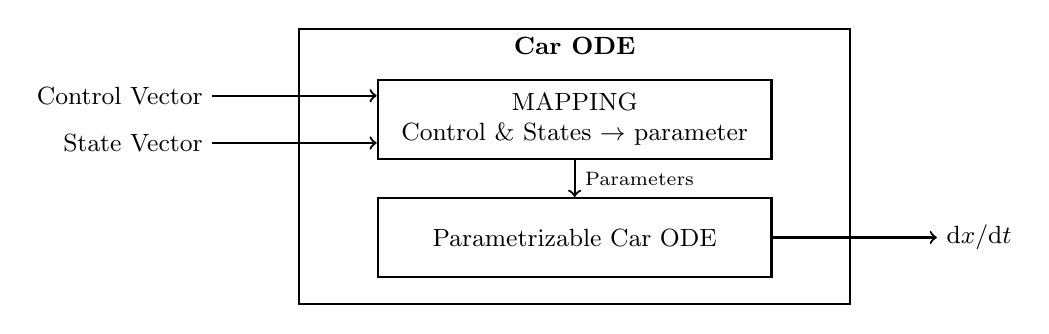
\begin{tikzpicture}[
			outerbox/.style={rectangle, draw, thick, minimum width=7cm, minimum height=3.5cm, align=center},
			innerbox/.style={rectangle, draw, thick, minimum width=5cm, minimum height=1cm, align=center, font=\small},
			arr/.style={->, thick},
		]

		\node[outerbox] (outer) at (0,0) {};
		\node[anchor=north, font=\small\bfseries] at (outer.north) {Car ODE};

		\node[innerbox] (mapping) at (0, 0.6) {MAPPING\\Control \& States $\to$ parameter};
		\node[innerbox] (carode)  at (0,-0.9) {Parametrizable Car ODE};

		\draw[arr] (mapping.south) -- (carode.north) node[midway, right, font=\scriptsize] {Parameters};

		% Inputs hug the outer box
		\node[anchor=east, font=\small] (ctrl)  at (-4.6,  0.9) {Control Vector};
		\node[anchor=east, font=\small] (state) at (-4.6,  0.3) {State Vector};
		\draw[arr] (ctrl.east)  -- (mapping.west |- ctrl.east);
		\draw[arr] (state.east) -- (mapping.west |- state.east);

		\node[anchor=west, font=\small] (out) at (4.6, -0.9) {$\mathrm{d}x/\mathrm{d}t$};
		\draw[arr] (carode.east) -- (out.west);

	\end{tikzpicture}
	\caption{Generic car model structure}
	\label{fig:generic_car}
\end{figure}


\subsection{Mass-point quasi-steady-state model}
A simple and useful car model can be built using these equations
\begin{align}
    F_z &= \tfrac{1}{2}\, \rho\, C_L\, v_x^2, \\
    F_y &= m\, v_x^2\, c, \\
    F_{x,\mathrm{pwr}} &= \frac{P_{\max}}{v_x}, \\
    F_{x,\max}^2 &= \max\!\left( \bigl[(F_z + m g)\mu\bigr]^2 - F_y^2,\; 0 \right), \\
    F_x^2 + F_y^2 &\le \bigl[(F_z + m g)\, \mu\bigr]^2, \\
    |F_x| &\le \min\!\bigl(F_{\mathrm{mot,max}},\; F_{x,\mathrm{pwr}}\bigr), \\
    \dot{v}_x &= \frac{F_x - \tfrac{1}{2}\, \rho\, C_D\, v_x^2}{m}.
    \label{QSS_model}
\end{align}
Here $\rho$ is the air density, $C_L$ is the lift coefficient, $v_x$ is the longitudinal speed, $m$ is the mass, $c$ is the curvature of the track at the current point, $P_{\max}$ is the maximum power of the motor, $\mu$ is the friction coefficient, and $C_D$ is the drag coefficient. This model has only one state, $v_x$, which makes it possible to use specialized lap-time simulation solvers. Variations of this model, where for example $P_{\max}$ is a lookup table or the grip does not scale linearly with down-force, are commonly used in motorsport.
\subsection{Single-track}
A more complex and useful model is the single-track model. In this model, suspension effects are neglected. The single-track model is still considered a simplified model and is used most commonly when more complex models are too computationally expensive. A computational graph of how this model is assembled from the defined components is shown in Figure~\ref{fig:singletrack}.
\begin{figure}[H]
	\centering
	\begin{tikzpicture}[
			box/.style={rectangle, draw, thick, fill=white, minimum width=2cm, minimum height=1.2cm, align=center, font=\small},
			smallbox/.style={rectangle, draw, fill=white, minimum width=1.5cm, minimum height=0.8cm, align=center, font=\scriptsize},
			arr/.style={->, thick},
			darr/.style={<->, thick},
		]

		% Car silhouette (background layer, top view: nose up, 4 wheels)
		\begin{scope}[on background layer]
			% main body (sedan proportions, length:width ~2:1)
			\fill[gray!12, draw=gray!40, line width=0.4pt, rounded corners=22pt]
				(-3.0, -6) rectangle (3.0, 5.5);
			% 2 wheels (centerline, large) — front wheel steered
			\begin{scope}[rotate around={20:(0,5)}]
				\fill[gray!45, draw=gray!60, rounded corners=6pt] (-1.4, 3.2) rectangle (1.4, 6.8);
			\end{scope}
			\fill[gray!45, draw=gray!60, rounded corners=6pt] (-1.4, -6.8) rectangle (1.4, -3.2);
		\end{scope}

		% CoG
		\node[box, minimum width=2.5cm, minimum height=1.5cm] (cog) at (0,0) {CoG};

		% Front tire (top = front of vehicle)
		\node[box] (tf) at (0, 5) {Tire\\Front};

		% Front wheel pivot between CoG and front tire
		\node[box] (waf) at (0, 2.5) {Wheel Pivot\\Front};

		% Rear wheel pivot between CoG and rear tire
		\node[box] (war) at (0, -2.5) {Wheel Pivot\\Rear};

		% Rear tire (bottom = rear of vehicle)
		\node[box] (tr) at (0, -5) {Tire\\Rear};

		% Front motor + gearbox (single box, inline right of front tire)
		\node[smallbox, minimum width=2cm] (mgf) at (3.5, 5) {Motor +\\Gearbox};

		% Rear motor + gearbox (single box, inline right of rear tire)
		\node[smallbox, minimum width=2cm] (mgr) at (3.5, -5) {Motor +\\Gearbox};

		% Aero
		\node[box] (aero) at (-4, 0) {Aero + static \\ suspension};

		% CoG <-> Front WA (velocity up, force down)
		\draw[arr] ($(cog.north)+(-0.3,0)$) -- node[left, font=\scriptsize] {$\symbf{v},\symbf{\omega}$} ($(waf.south)+(-0.3,0)$);
		\draw[arr] ($(waf.south)+(0.3,0)$) -- node[right, font=\scriptsize] {$\symbf{F},\symbf{M}$} ($(cog.north)+(0.3,0)$);

		% CoG <-> Rear WA
		\draw[arr] ($(cog.south)+(-0.3,0)$) -- node[left, font=\scriptsize] {$\symbf{v},\symbf{\omega}$} ($(war.north)+(-0.3,0)$);
		\draw[arr] ($(war.north)+(0.3,0)$) -- node[right, font=\scriptsize] {$\symbf{F},\symbf{M}$} ($(cog.south)+(0.3,0)$);

		% Front WA <-> Front Tire (velocity up, force down)
		\draw[arr] ($(waf.north)+(-0.3,0)$) -- node[left, font=\scriptsize] {$\symbf{v}_{tire}$} ($(tf.south)+(-0.3,0)$);
		\draw[arr] ($(tf.south)+(0.3,0)$) -- node[right, font=\scriptsize] {$\symbf{F}_{tire}$} ($(waf.north)+(0.3,0)$);

		% Rear WA <-> Rear Tire
		\draw[arr] ($(war.south)+(-0.3,0)$) -- node[left, font=\scriptsize] {$\symbf{v}_{tire}$} ($(tr.north)+(-0.3,0)$);
		\draw[arr] ($(tr.north)+(0.3,0)$) -- node[right, font=\scriptsize] {$\symbf{F}_{tire}$} ($(war.south)+(0.3,0)$);

		% Motor + Gearbox -> Tire (front)
		\draw[arr] (mgf.west) -- node[above, font=\scriptsize] {$T_{out}$} (tf.east);

		% Motor + Gearbox -> Tire (rear)
		\draw[arr] (mgr.west) -- node[above, font=\scriptsize] {$T_{out}$} (tr.east);

		% Aero -> CoG
		\draw[arr] (aero.east) -- node[above, font=\scriptsize] {$F_{drag}$} (cog.west);

		% Aero -> Tires (Fz via downforce)
		\draw[arr] (aero.north) -- (-4, 7.3) -- node[above, font=\scriptsize] {$F_z$} (0, 7.3) -- (tf.north);
		\draw[arr] (aero.south) -- (-4, -7.3) -- node[below, font=\scriptsize] {$F_z$} (0, -7.3) -- (tr.south);

		% Steering input
		\draw[arr] (-3, 5) -- node[above, font=\scriptsize] {$\delta$} (tf.west);

		% States out of CoG
		\draw[arr] (cog.east) -- node[above, font=\scriptsize] {$\symbf{x} = [v_x,\, v_y,\, \dot\psi,\, \psi]^T$} (5.5, 0);

	\end{tikzpicture}
	\caption{Single-track (bicycle) model}
	\label{fig:singletrack}
\end{figure}

\subsection{Twin-track model}
The twin-track model treats all four tires separately. This captures the left-right load transfer. The computational graph is shown in Figure~\ref{fig:twintrack}.
\begin{figure}[H]
	\centering
	\begin{tikzpicture}[
			box/.style={rectangle, draw, thick, fill=white, minimum width=1.7cm, minimum height=0.9cm, align=center, font=\scriptsize},
			smallbox/.style={rectangle, draw, fill=white, minimum width=1.4cm, minimum height=0.7cm, align=center, font=\tiny},
			arr/.style={->, thick},
		]

		\begin{scope}[on background layer]
			\fill[gray!12, draw=gray!40, line width=0.4pt, rounded corners=22pt]
				(-4.0, -6) rectangle (4.0, 5.5);
			\begin{scope}[rotate around={20:(-3,5)}]
				\fill[gray!45, draw=gray!60, rounded corners=6pt] (-3.6, 3.2) rectangle (-2.4, 6.8);
			\end{scope}
			\begin{scope}[rotate around={20:(3,5)}]
				\fill[gray!45, draw=gray!60, rounded corners=6pt] (2.4, 3.2) rectangle (3.6, 6.8);
			\end{scope}
			\fill[gray!45, draw=gray!60, rounded corners=6pt] (-3.6, -6.8) rectangle (-2.4, -3.2);
			\fill[gray!45, draw=gray!60, rounded corners=6pt] (2.4, -6.8) rectangle (3.6, -3.2);
		\end{scope}

		% CoG
		\node[box, minimum width=2.4cm, minimum height=1.4cm] (cog) at (0,0) {CoG};

		% Wheel pivots
		\node[box] (wafl) at (-3, 2.5) {Wheel Pivot\\FL};
		\node[box] (wafr) at ( 3, 2.5) {Wheel Pivot\\FR};
		\node[box] (warl) at (-3,-2.5) {Wheel Pivot\\RL};
		\node[box] (warr) at ( 3,-2.5) {Wheel Pivot\\RR};

		% Tires
		\node[box] (tfl) at (-3, 5) {Tire FL};
		\node[box] (tfr) at ( 3, 5) {Tire FR};
		\node[box] (trl) at (-3,-5) {Tire RL};
		\node[box] (trr) at ( 3,-5) {Tire RR};

		% Motors
		\node[smallbox] (mgfl) at (-5.5, 5) {Motor+GB\\FL};
		\node[smallbox] (mgfr) at ( 5.5, 5) {Motor+GB\\FR};
		\node[smallbox] (mgrl) at (-5.5,-5) {Motor+GB\\RL};
		\node[smallbox] (mgrr) at ( 5.5,-5) {Motor+GB\\RR};

		% Aero (left) and Suspension (right)
		\node[box] (aero) at (-7, 0) {Aero};
		\node[box] (susp) at ( 7, 0) {Suspension};

		% CoG <-> wheel pivots
		\foreach \wp in {wafl, wafr, warl, warr}{%
			\draw[arr] (cog) -- (\wp);
			\draw[arr] (\wp) -- (cog);
		}

		% Wheel pivot <-> tire
		\draw[arr] (wafl) -- (tfl); \draw[arr] (tfl) -- (wafl);
		\draw[arr] (wafr) -- (tfr); \draw[arr] (tfr) -- (wafr);
		\draw[arr] (warl) -- (trl); \draw[arr] (trl) -- (warl);
		\draw[arr] (warr) -- (trr); \draw[arr] (trr) -- (warr);

		% Motors -> tires
		\draw[arr] (mgfl.east) -- node[above, font=\tiny] {$T_{out}$} (tfl.west);
		\draw[arr] (mgfr.west) -- node[above, font=\tiny] {$T_{out}$} (tfr.east);
		\draw[arr] (mgrl.east) -- node[above, font=\tiny] {$T_{out}$} (trl.west);
		\draw[arr] (mgrr.west) -- node[above, font=\tiny] {$T_{out}$} (trr.east);

		% Aero -> CoG
		\draw[arr] (aero.east) -- node[above, font=\tiny] {$F_{drag}, F_{lift}$} (cog.west);

		% Suspension <-> all 4 wheel pivots (bidirectional: F_susp into pivot, displacement back)
		\foreach \wp in {wafl, wafr, warl, warr}{%
			\draw[arr] (susp) -- (\wp);
			\draw[arr] (\wp) -- (susp);
		}

		% Steering
		\draw[arr] (-5, 6.5) -- node[above, font=\tiny] {$\delta_{FL}$} (tfl.north west);
		\draw[arr] ( 5, 6.5) -- node[above, font=\tiny] {$\delta_{FR}$} (tfr.north east);

		% State vector — straight down from CoG
		\node[below=2.2cm of cog, font=\scriptsize, align=center] (statevec)
			{$\symbf{x} = [v_x,\, v_y,\, \dot\psi,\, \psi]^T$};
		\draw[arr] (cog.south) -- (statevec.north);

	\end{tikzpicture}
	\caption{Twin-track model}
	\label{fig:twintrack}
\end{figure}


\section{Track modeling}
The track is sampled at discrete arc length nodes $s_i$ and stored as a set of
fields evaluated at each node:
\begin{itemize}
	\item centerline coordinates $x(s)$, $y(s)$,
	\item heading $\theta(s)$,
	\item curvature $\kappa(s)$,
	\item left and right track widths $w_L(s)$, $w_R(s)$,
	\item air density $\rho(s)$,
	\item friction coefficient $\mu(s)$,
	\item inclination $\phi(s)$.
\end{itemize}
Each field is linearly interpolated between the segments. Obtaining a suitable track for optimization from GPS is non-trivial. Simple methods lead to noisy data, which then corrupts the optimization result. Therefore, the smoothing method described in \cite{perantoniOptimalControlFormula2014} has been used.

\section{Change of independent variable, time to path}
When the differential equations for vehicle movement are stated, it is
beneficial in lap time simulation to describe the car states not in time but in
distance travelled. This introduces a connection with the location on the
track and reduces the number of state variables by one. This transformation is
taken from \cite{perantoniOptimalControlFormula2014}.

\begin{equation}
	\varepsilon = \psi - \theta(s)
\end{equation}
where $\psi$ is the car heading, and $\theta(s)$ is the heading of the track at distance $s$.

\begin{equation}
	S_f = \frac{\mathrm{d}t}{\mathrm{d}s} = \frac{1 - n\, C(s)}{v_x \cos\varepsilon - v_y \sin\varepsilon},
	\label{time2path}
\end{equation}

$n$ is the vehicle's distance from the centerline, and $C(s)$ is the curvature of the track at distance~$s$. The change in $n$ is defined as:
\begin{equation}
	\frac{\mathrm{d}n}{\mathrm{d}t} = v_x \sin\varepsilon + v_y \cos\varepsilon.
\end{equation}
Then the model can be transformed from time as the independent variable to distance travelled along the centerline $s$ as the new independent variable using the equation:
\begin{equation}
	\frac{\mathrm{d}}{\mathrm{d}s}
	\begin{pmatrix} v_x \\ v_y \\ \psi \\ \dot{\psi} \\ n \\ t \end{pmatrix}
	=
	S_f
	\begin{pmatrix}
		\dot{v}_x    \\
		\dot{v}_y    \\
		\dot{\psi}   \\
		\ddot{\psi} \\
		\dot{n}      \\
		1
	\end{pmatrix}.
\end{equation}
\begin{figure}[H]
	\centering
	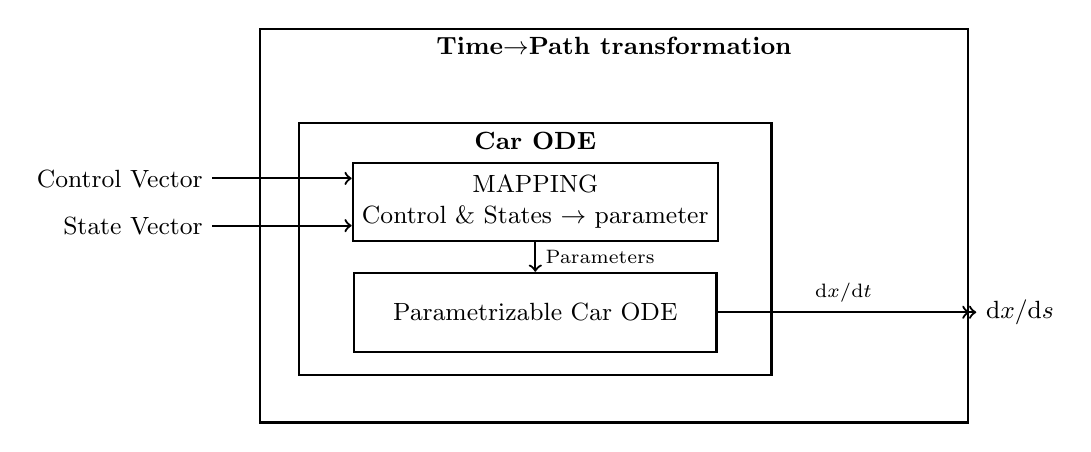
\begin{tikzpicture}[
			outermost/.style={rectangle, draw, thick, minimum width=9cm, minimum height=5cm, align=center},
			outerbox/.style={rectangle, draw, thick, minimum width=6cm, minimum height=3.2cm, align=center},
			innerbox/.style={rectangle, draw, thick, minimum width=4.6cm, minimum height=1cm, align=center, font=\small},
			arr/.style={->, thick},
		]

		\node[outermost] (wrap) at (0,0) {};
		\node[anchor=north, font=\small\bfseries] at (wrap.north) {Time$\to$Path transformation};

		\node[outerbox] (outer) at (-1.0, -0.3) {};
		\node[anchor=north, font=\small\bfseries] at (outer.north) {Car ODE};

		\node[innerbox] (mapping) at (-1.0, 0.3)  {MAPPING\\Control \& States $\to$ parameter};
		\node[innerbox] (carode)  at (-1.0,-1.1)  {Parametrizable Car ODE};

		\draw[arr] (mapping.south) -- (carode.north) node[midway, right, font=\scriptsize] {Parameters};

		\node[anchor=east, font=\small] (ctrl)  at (-5.1, 0.6) {Control Vector};
		\node[anchor=east, font=\small] (state) at (-5.1, 0.0) {State Vector};
		\draw[arr] (ctrl.east)  -- (mapping.west |- ctrl.east);
		\draw[arr] (state.east) -- (mapping.west |- state.east);

		\draw[arr] (carode.east) -- node[above, font=\scriptsize] {$\mathrm{d}\symbf{x}/\mathrm{d}t$} (wrap.east |- carode.east);

		\node[anchor=west, font=\small] (out) at (4.6, -1.1) {$\mathrm{d}\symbf{x}/\mathrm{d}s$};
		\draw[arr] (wrap.east |- out.west) -- (out.west);

	\end{tikzpicture}
	\caption{Car with a time-to-path transformation layer}
	%\label{fig:generic_car_t2p}
	\label{fig:generic_car_t2p}
\end{figure}

Now the vehicle is modeled and placed on the track. The next step is to drive it as fast as possible.